\documentclass[tikz,border=10pt]{standalone}
\usepackage[T1]{fontenc}
\usepackage{lmodern}
\usetikzlibrary{positioning,arrows.meta,fit}

\begin{document}
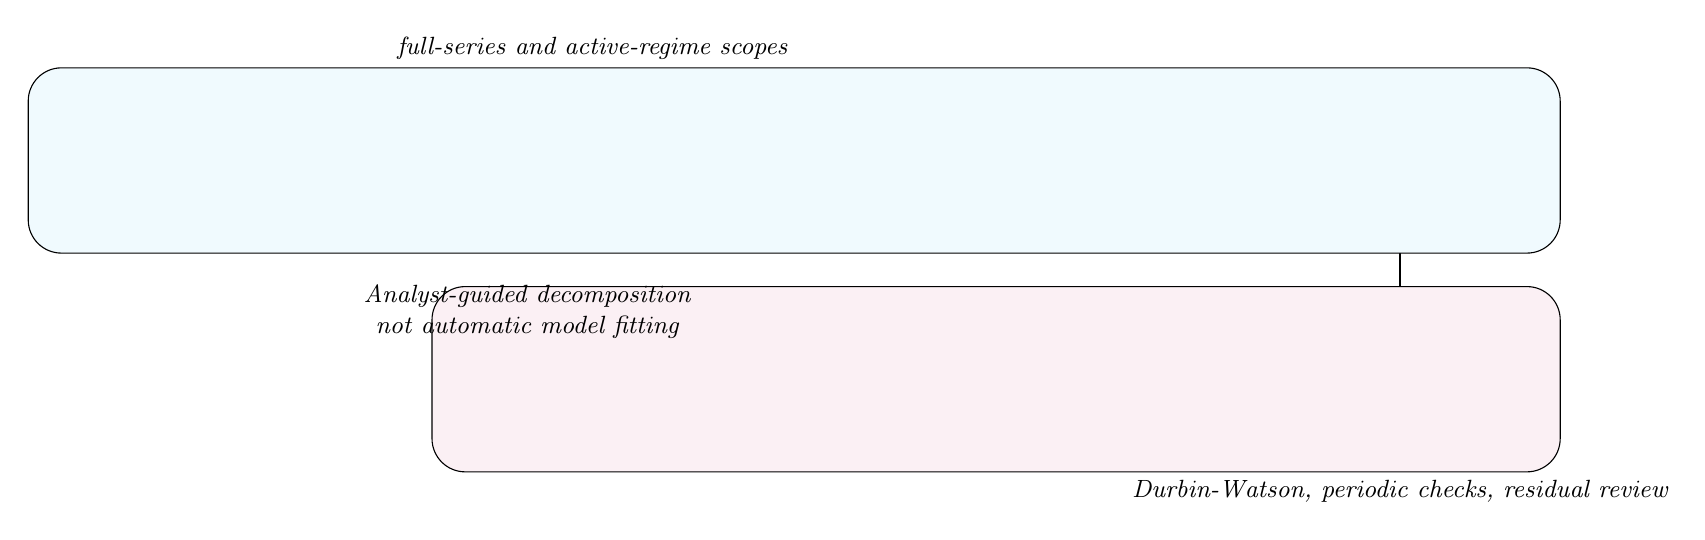
\begin{tikzpicture}[
  box/.style={draw, rounded corners=8pt, align=center, minimum width=3.2cm, minimum height=1.2cm, fill=blue!8, line width=0.8pt},
  accent/.style={draw, rounded corners=8pt, align=center, minimum width=3.2cm, minimum height=1.2cm, fill=green!10, line width=0.8pt},
  note/.style={font=\small\itshape, align=center},
  arrow/.style={-Latex, thick, shorten >=2pt, shorten <=2pt}
]

% Flow nodes
\node[box] (raw) {Raw\\series};
\node[box, right=1.9cm of raw] (assess) {Initial\\assessment};
\node[box, right=1.9cm of assess] (window) {Window\\selection};
\node[box, right=1.9cm of window] (group) {Component\\grouping};
\node[box, below=1.55cm of group] (validate) {Validation\\\& diagnostics};
\node[accent, left=1.9cm of validate] (report) {Observation\\logging};
\node[accent, left=1.9cm of report] (decision) {Audit-ready\\report};

% Scope / regime notes
\node[note, above=0.55cm of assess] {full-series and active-regime scopes};
\node[note, below=0.55cm of validate] {Durbin-Watson, periodic checks, residual review};

% Connectors
\draw[arrow] (raw) -- (assess);
\draw[arrow] (assess) -- (window);
\draw[arrow] (window) -- (group);
\draw[arrow] (group) -- (validate);
\draw[arrow] (validate) -- (report);
\draw[arrow] (report) -- (decision);

\node[draw, rounded corners=12pt, fit=(raw) (assess) (window) (group), inner xsep=12pt, inner ysep=16pt, fill=cyan!6] {};
\node[draw, rounded corners=12pt, fit=(validate) (report) (decision), inner xsep=12pt, inner ysep=16pt, fill=purple!6] {};

\node[note, align=center, below=0.85cm of raw, xshift=4.3cm] {Analyst-guided decomposition\\not automatic model fitting};

\end{tikzpicture}
\end{document}
